\section{Combinational Logic}

\subsection{Static complementary CMOS}

\begin{wrapfigure}{r}{0.5\textwidth}
    \centering
    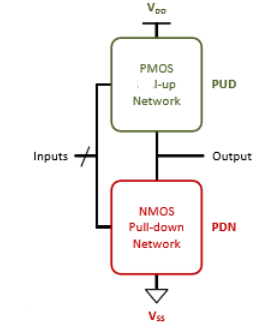
\includegraphics[scale=1.0]{images/static_CMOS.png}
    \caption{Static CMOS}
\end{wrapfigure}

\begin{wrapfigure}{l}{0.7\textwidth}
    \centering
    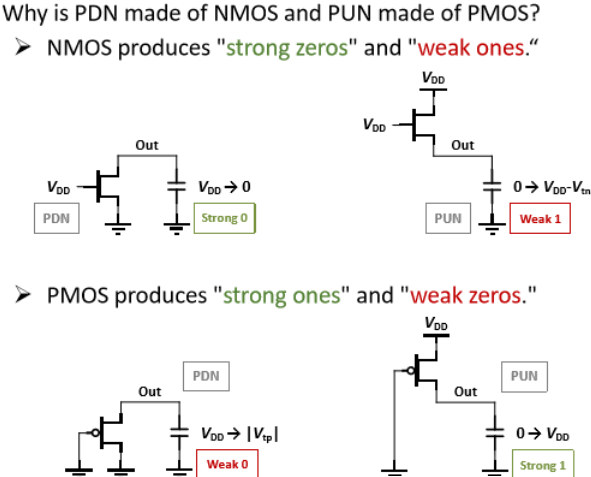
\includegraphics[scale=0.7]{images/PDN_PUN_NMOS_PMOS.png}
    \caption{PDN and PUN}
\end{wrapfigure}

\begin{itemize}
    \item Pull-up Network (PUN): Constructed using PMOS transistors
    \item Pull-down Network (PDN): Constructed using NMOS transistors
\end{itemize}

PUN and PDN are dual logic networks. One and only one of the networks conduct at DC. 